\documentclass[a4paper,fleqn]{cas-dc}
\usepackage[numbers]{natbib}
\usepackage{caption}
\captionsetup{labelformat=simple, labelsep=colon}
\usepackage{float}
\usepackage{mathtools}
\usepackage{booktabs}
\usepackage{placeins}
\usepackage{flushend}
\usepackage{graphicx}
\usepackage{algorithm}
\usepackage{algorithmic}
\usepackage{amsmath}
\usepackage{amssymb}  
\usepackage{tikz}
\usepackage{subcaption}
\usepackage{array}

\usepackage{chngcntr}
\counterwithin{figure}{subsection}

\numberwithin{equation}{section}

\begin{document}
\let\WriteBookmarks\relax
\def\floatpagepagefraction{1}
\def\textpagefraction{.001}

\shorttitle{Cross-Layer QoS Optimization for High-Reliability WSN-based IoT Networks}
\shortauthors{S Gopikrishnan et~al.}

\title [mode = title]{Cross-Layer QoS Optimization for High-Reliability WSN-based IoT Networks}                      


%Name: D Boja Bindusri
%Reg.No.: 23MIC7266
%gmail: bojabindusri@gmail.com
%Email: bindusri.23mic7266@vitapstudent.ac.in
%orcid: 0009-0002-8545-7095



\author[1]{ D Boja Bindusri}[orcid=0009-0002-8545-7095]
\ead{bindusri.23mic7266@vitapstudent.ac.in}
\address[1]{School of Computer Science and Engineering, VIT-AP University, Amaravathi. Andhra Pradesh, India}



\cortext[cor1]{Corresponding author}

\begin{abstract}
The rapid expansion of Internet of Things environments has introduced significant challenges in maintaining reliable and energy-efficient communication in wireless sensor networks. Dynamic network conditions such as congestion, link instability, and energy depletion adversely affect Quality of Service performance. To address these issues, this work proposes a Cross Layer Quality of Service Adaptive Decision Support System for wireless sensor network based Internet of Things networks. The proposed framework integrates parameters from physical, medium access control, and network layers, including residual energy, link quality, delay, and traffic load, to enable adaptive and intelligent routing decisions. A multi-metric cost function is employed to select optimal forwarding nodes, while load balancing mechanisms ensure efficient energy utilization across the network. The system dynamically adapts routing paths based on real-time network conditions, improving reliability and stability. Simulation results demonstrate that the proposed approach achieves higher packet delivery ratio, lower delay, improved throughput, and enhanced network lifetime compared to existing routing methods. The proposed model provides a scalable and efficient solution for reliable data transmission in dynamic wireless sensor network based Internet of Things environments.

\end{abstract}

\begin{keywords}
Wireless Sensor Networks \sep 
Internet of Things (IoT) \sep 
Cross Layer Optimization \sep 
Quality of Service \sep
Energy Efficiency \sep 
Routing Protocol
\end{keywords}

\maketitle



\section{Introduction}
WSN-based IoT networks are used in smart cities, healthcare, agriculture and industrial monitoring. There, the data collected by sensor nodes is sent to a sink for processing. Since these devices only have a limited battery life, we need to select paths that save power to keep the whole network alive for as long as possible. Network conditions keep changing in large IoT deployments due to congestion, traffic variation, weak links, etc. Therefore, cross-layer information from the physical, MAC, and network layers is required to maintain quality of service (QoS) and reliability. Classical routing methods may lead to packet loss and early node failure. However, for high-reliability, packet loss must be low and consistent packet delivery should be maintained. Heterogeneous routing helps by using nodes with different energy levels, but still finding the best route is critical. Hence, an Adaptive Decision Support System-based heterogeneous routing protocol chooses energy-saving routes by considering residual energy, distance, link quality, and QoS needs.

\subsection{Need of adaptive decision support for WSN-based IoT network}
 
In WSN-based IoT environments node energy level decreases,  packet traffic changes over time, and communication links degrade due to factors such as interference, mobility, or obstacles. As a result, static routing choices cannot maintain stable performance. This can cause latency, reduced performance, and early node death. The Adaptive Decision Support System (ADDS) supports cross-layer QoS optimization using updated parameters from multiple layers. DSS-based routing provides better QoS performance in IoT networks by improving accuracy and avoiding poor route selections.


\subsection{Research Objectives}

The main aim of this research is to extend the lifetime of WSN-based IoT networks and lower power consumption. The objective focuses on improving energy efficiency so that the network can operate for a longer duration under an extremely low power budget. To optimize the selection of cluster heads through energy stabilization, distance reduction, and latency minimization between nodes. This objective also aims to determine shortest and efficient routes while dynamically minimizing network overhead during network operation.

To develop a cross-layer QoS-aware routing framework to improve the Quality of Service in data transmission. This includes evaluating and improving packet delivery ratio (PDR), packet delay, throughput, network lifetime, packet loss rate, and error estimation while maintaining the required reliability. To incorporate cross-layer routing and power control mechanisms for reliable multi-path transmission while maintaining a manageable conflict probability. This objective also aims to enhance key network metrics such as SNR, residual energy, and link quality estimation to support stable and reliable end-to-end communication under dynamic conditions like mobility.


\section{Literature Survey}
The research \cite{eljakani2025predicting} on the dynamic field of IoT applications based on the IEEE 802.15.4 standard clearly shows that balancing SNR, MGP, EC, and PDR is vital. We introduced novel control parameters at the application layer, effectively working with the dynamic MLP architecture and the adaptable WES loss function to maintain an optimal trade-off between these QoS metrics. This approach improved prediction accuracy across various scenarios, achieving an average of 97 percent across the R-squared of all the QoS metrics, showcasing the model’s adaptability. WSNs are \cite{obaid2024optimizing}composed of nodes with limited resources that deal with a variety of issues. One such difficulty is network congestion, which primarily results from a node’s receipt rate exceeding its transmission rate. It is determined that congestion cannot be detected by a single metric. For accurately identifying congestion,  multiple metrics must be employed. Energy-efficient congestion management techniques are necessary in WSNs and guaranty minimal energy usage, fairness, and significantly improved quality of service.

\subsection{AI-Driven Cross-Layer Optimization for Resource Allocation, Routing, and Congestion Control in WSN-IoT Networks}
A DRL-based radio\cite{huang2023drl} resource allocation approach for joint scheduling and precoding in a massive MIMO system is investigated. The method decomposes the cross-layer adaptation decision by combining multiple algorithms and learns selection policy in challenging 5G traffic scenarios. The proposed algorithm selection supports decision-making and serves as a smart agent in future mobile networks. The CLCQ \cite{he2024cross}effectively integrates the information from the physical layer and data link layer to intelligently select the next hop node. This function considers various factors, including channel quality, buffer state, and residual energy, in order to select the optimal route for forwarding data packets. Finally, the comparison of the CLCQ with QELAR and GEDAR shows that the CLCQ has clear advantages in energy consumption control, delay reduction, and delivery rate improvement in large-scale networks.

In this study\cite{sefati2025intelligent}, we present a hybrid GAN-ACO congestion control framework for WSNs aimed at enhancing energy efficiency, latency reduction, and reliability. Utilizing GANs for efficient cluster formation and ACO for adaptive routing, this approach balances load distribution while dynamically responding to congestion through pheromone-based path selection. The simulation results demonstrate that GAN-ACO consistently surpasses existing congestion control methods across key QoS metrics—particularly in terms of energy conservation, reduced latency, and higher reliability.This paper\cite{zheng2025ai} has presented a comprehensive study on AI-driven resource management for heterogeneous IIoT systems. Based on these insights, a unified AI-driven resource management framework has been proposed, integrating sensing, prediction, and optimization through synergistic AI paradigms including DL, DRL, FL, LLM, and GenAI.This paper presented \cite{fan2025optimizing} the SAC-IRS algorithm, a novel approach combining Intelligent Reflecting Surfaces (IRS) and Reinforcement Learning (RL) to optimize network performance. The proposed algorithm leverages dynamic IRS phase shifts at the physical layer, and implements cross-layer optimization to enhance packet delivery rates and energy efficiency.

This review paper\cite{thakur2025ai} highlights the existing routing algorithms from classic to AI approaches and shows a critical role in IoT-based WSN applications and the growing need for energy-efficient (EE) protocols to enhance network lifespan and throughput. By evaluating both, the survey highlights how static routing methods fall short in dynamic environments and how intelligent optimization methods tackle scalability, reliability, and energy constraints.This research \cite{peng2025two} have investigated the two-timescale cross layer design in the FBL regime for URLLC by jointly considering large timescale pilot length and pilot power optimization and small timescale data transmission adaptation. A TD3-based DRL algorithm was utilized to adaptively determine the instantaneous transmit power on different sub-channels and the decoding error probability in an ideal environment with known perfect CSI, aiming to minimize the average data transmit power.

\subsection{Cross-Layer and AI-Enabled URLLC Resource Management for 6G IoT Networks}
This paper\cite{ibrahim2025urllc} has reviewed URLLC solutions for 6G enabled Industry 5.0 through a structured taxonomy linking applications, enabling technologies, design challenges, and performance enhancements. However, open issues remain in areas such as zero slack security, scalable channel estimation for RIS, adaptive orchestration across heterogeneous edge resources, and energy informed mobility management.This study introduced \cite{andong2025federated} FERMI-6G, a federated multi agent reinforcement learning framework for decentralized, privacy-preserving, and energy-aware resource management in ultra-dense 6G edge networks. FERMI-6G enables agents to jointly optimize task offloading, spectrum access, and CPU scaling under partial observability and mobility constraints. Experimental results showed that FERMI-6G surpasses existing baselines in reliability, latency, energy efficiency, and scalability while preserving privacy.

Cross layer based energy aware path scheduling algorithm\cite{jenila2023cross} is proposed to reduce congestion ratio and to improve link quality between the routing nodes. Semi-Markov process is applied for estimating link quality among nodes as well as its durability. Simulation analysis is carried out through network simulator tool and the proposed mechanism efficacy is compared with the conventional schemes. Proposed scheme shows better results with improved performance.Cross Layer Design (CLD) \cite{ghushe2023cross}can be utilized to further enhance a number of IoT features and increase system’s efficiency. This paper provides a detailed discussion of the IoT’s evolution, communication technologies, and applications. When combined with IoT, a number of proposed CLDs had different issues that were solved based on concerns about security, privacy, mobility, interoperability, and energy consumption. Although this study has explored a number of potential solutions, different approaches that might be taken to address IoT-related issues are still required.

This study proves \cite{zhang2025edge} that ECSM is the best paradigm to use to realize ultra-low latency, energy efficiency, and scalability of smart city IoT networks. The hybrid approach, which combines local processing at the edge with global analytics at the cloud, eliminates the shortcomings of conventional architectures and provides real-time responsiveness in a range of applications - traffic management and telemedicine, disaster response. This paper \cite{qin2025routing} reviewed representative work on WBAN routing protocols and addressed the three research questions stated in the introduction. For RQ3, we summarized open issues, including adaptive multi-objective weighted optimization and robustness under highly dynamic conditions, and discussed AI, edge computing, and 6G-related technologies as potential future research directions. 


\begin{table*}[h]
\centering
\renewcommand{\arraystretch}{1.2}
\setlength{\tabcolsep}{4pt}
\caption{Literature Survey Table }
\label{tab:lit_survey}
\begin{tabular}{|c|p{3.7cm}|p{4.5cm}|p{4.5cm}|p{3.7cm}|}
\hline
\textbf{Ref.} & \textbf{Method Proposed} & \textbf{Techniques Used} & \textbf{Issues Resolved} & \textbf{Limitation} \\
\hline

R16 & Integrated cross-layer QoS measurement framework for 5G-enabled smart infrastructure \cite{balvad2025integrated}& Cross-layer monitoring, active--passive QoS measurement, network analytics, AI-assisted correlation & Improves service reliability, latency prediction accuracy, and holistic QoS assessment across layers & Focuses on QoS measurement rather than QoS optimization or control \\
\hline

R17 & Low-latency adaptive communication protocol (MLACP) for ultra-dense networks \cite{he2025low}& Cross-layer control, RNN-based state prediction, DQN optimization, dynamic resource slicing & Reduces end-to-end latency, packet loss, and improves throughput and stability & Scalability to large-scale IoT and WSN environments is not fully evaluated \\
\hline

R18 & UE-side cross-layer metrics framework for Zero-Touch network management \cite{tarrias2023ue}& UE-side metrics, cross-layer KPIs, machine learning-based analytics & Enhances automated network management, QoE awareness, and scalability & Dependence on UE-side data availability and potential privacy concerns \\
\hline

R19 & Cross-layer survey on secure and low-latency communications in next-generation IoT \cite{martalo2024cross}& Access, network, and application layer analysis, QUIC-based solutions & Identifies joint security and latency challenges and cross-layer solutions & Does not provide a concrete optimization framework or implementation\\
\hline

R20 & QoS-aware hybrid MAC protocol for real-time Wi-Fi~8 (IEEE~802.11bn) networks \cite{bt5276263qos}& Federated reinforcement learning, TSN-based deterministic scheduling, cross-layer feedback & Achieves ultra-low latency, bounded jitter, and high reliability for real-time traffic & Primarily designed for Wi-Fi~8; limited applicability to WSN-based IoT networks \\
\hline

R21 & Digital Twin as a Service (DTaaS) architecture for predictive slice management in 6G \cite{bilen2025modular}& Digital twins, deep sequential models, cross-layer telemetry, predictive orchestration & Improves SLA compliance, proactive resource provisioning, and slice reliability & High architectural complexity and computational overhead \\
\hline

R22 & Machine learning-driven optimization of 5G network slicing for URLLC road safety analytics \cite{dlamini2024enhancing}& Network slicing, ML-based resource allocation, cross-layer orchestration & Achieves ultra-low latency and improved reliability for safety-critical V2X services & Limited to vehicular road safety use cases; general IoT applicability is not validated \\
\hline

R23 & Secure and reliable multi-objective optimized multipath transmission (MOMTA-HN)\cite{qi2024momta} & Multi-objective optimization, ONSGA-II, multipath routing, deletion graph & Improves reliability, security, and low-latency transmission under network attacks and failures & High computational complexity and increased signaling overhead \\
\hline

R24 & Edge--cloud synergy model for ultra-low latency smart city IoT networks \cite{zhang2025edge}& Edge computing, cloud computing, network slicing, AI-based resource management & Reduces end-to-end latency and improves QoS and service reliability & Requires complex orchestration and interoperability across layers \\
\hline

R25 & Quantum machine intelligence framework for 6G URLLC \cite{zaman2023quantum}& Quantum machine learning, DRL, federated learning, variational quantum algorithms & Addresses learning latency and optimization challenges in URLLC scenarios & Dependency on quantum hardware and lack of practical deployment feasibility \\
\hline

R26 & Comprehensive survey of URLLC solutions for 5G and 6G networks \cite{haque2025comprehensive}& PHY, MAC, and cross-layer techniques, machine learning-based optimization & Systematic analysis of latency--reliability trade-offs and open research challenges & Survey-oriented; lacks experimental validation \\
\hline

R27 & QoS-aware deep reinforcement learning-based link adaptation (QDRLLA) \cite{parsa2025qos}& Deep reinforcement learning, adaptive MCS selection, power control, OFDM numerology & Enhances QoS satisfaction in terms of latency, reliability, and throughput & High training complexity and dependency on accurate state information \\
\hline

R28 & Cross-layer channel estimation-aware routing protocol for IIoT \cite{salih2023dynamic}& Cross-layer routing, channel availability probability, cognitive radio sensing & Improves packet delivery ratio, throughput, and routing stability & Increased control overhead and complexity in highly mobile environments \\
\hline

R29 & Intelligent path management for heterogeneous vehicular networks \cite{singh2025study}& MPTCP, FAHP-based network selection, multipath connectivity & Improves service continuity and reliability during vertical handovers & Energy efficiency and WSN constraints are not explicitly addressed \\
\hline

R30 & Study of advanced routing and packet compression for WBANs \cite{hapanchak2024intelligent}& Energy-efficient routing, packet compression techniques & Enhances energy efficiency, throughput, and communication reliability & Not suitable for large-scale or highly dynamic IoT deployments \\
\hline

\end{tabular}
\end{table*}
\clearpage

\subsection{Research gaps and Motivation}
\subsubsection{Research gaps}
Existing cross-layer routing protocols in WSN-based IoT networks primarily rely on static weighting mechanisms and limited parameter consideration. These approaches fail to dynamically adapt to real-time variations in traffic load, energy depletion, and link quality, especially in dense and large-scale deployments. As a result, routing decisions become inefficient under dynamic conditions, leading to reduced packet delivery ratio, increased delay, and unbalanced energy consumption.

Furthermore, most existing methods focus on single-path routing and do not effectively consider adaptive decision-making based on real-time network conditions. The lack of dynamic parameter adjustment limits their performance in highly dynamic IoT environments. Therefore, there is a need for an adaptive cross-layer routing framework that dynamically adjusts routing parameters based on real-time network conditions to improve QoS and energy efficiency.
\subsubsection{Motivation}
The existing cross-layer-based opportunistic routing protocol (CORP) algorithm has several drawbacks: High data transmission complexity occurs when the number of constraints increases due to the limited computing power of the WSNs. Results have yet to be found so far that satisfy the real-time demands of WSNs. There isn't much discussion of QoS studies centered on WBAN applications in the literature. QoS-Aware Wireless sensor network routing protocols have been developed, however no QoS-based standard routing method has been developed for WBAN. However, these routing protocols do not optimize the route selection by taking into account critical network conditions such as channel diversity, interference and QoS requirements for WBAN. Hence, this motivates the need for a cross-layer QoS optimization approach to achieve high reliability and real-time QoS performance in WSN-based IoT networks.
Therefore, to address these limitations, this work proposes an adaptive cross-layer QoS optimization framework that dynamically adjusts routing decisions based on real-time network conditions such as energy levels, traffic load, and link quality. The proposed approach aims to improve reliability, reduce delay, and enhance overall network performance in dynamic WSN-based IoT environments.

\section{Problem Statement}
WSN-based IoT networks are widely used in critical applications such as agriculture, industrial monitoring, smart healthcare, and smart city infrastructure, where reliable and timely data delivery is essential. However, sensor nodes operate under strict energy and processing constraints, and the network is affected by dynamic traffic, congestion, interference, and unstable wireless links. These challenges significantly degrade Quality of Service (QoS) metrics such as packet delivery ratio, delay, throughput, and network lifetime.

Most existing approaches focus on single-layer optimization and consider only limited network parameters, which restricts their ability to adapt to dynamic environments and maintain reliable communication. As a result, these methods fail to provide consistent performance under varying network conditions. Therefore, there is a need for a cross-layer QoS optimization framework that integrates multiple protocol layers to improve reliability, energy efficiency, and stable data transmission in WSN-based IoT networks.

\section{Proposed Work}
To address the limitations of existing routing approaches, this work proposes a Cross-Layer QoS Adaptive Decision Support System (CL-QoS-ADDS) for WSN-based IoT networks. The proposed system integrates parameters from physical, MAC, and network layers to enable intelligent and adaptive routing decisions under dynamic conditions.

The framework focuses on improving key QoS metrics such as packet delivery ratio, delay, throughput, and energy efficiency by dynamically selecting optimal routing paths based on real-time network conditions.
The proposed system considers a Wireless Sensor Network (WSN)-based IoT environment deployed over a two-dimensional monitoring area. Let the sensing region be represented by a square area A of size L×L.
A set of N sensor nodes is randomly distributed within the sensing field. These sensor nodes are responsible for collecting environmental data such as temperature, humidity, or other application-specific parameters.

The network consists of the following components:
N sensor nodes
One sink node (base station)
Multiple cluster heads

The sink node is assumed to have unlimited energy resources and higher processing capability compared to the sensor nodes. It acts as the final destination for all sensed data collected from the network. The sensor nodes communicate with the sink node using multi-hop communication, where intermediate nodes forward the packets.


\subsection{Network Model}
The proposed system considers a wireless sensor network based Internet of Things environment represented as a graph structure, where sensor nodes communicate through wireless links to deliver sensed data to a sink node. The network operates under strict energy constraints, limited bandwidth, and dynamic channel conditions. To address these challenges, the proposed model incorporates cross layer information to support adaptive and intelligent routing decisions. Nodes communicate using multi hop transmission, where intermediate nodes assist in forwarding data efficiently towards the sink.


\subsubsection{Network Deployment}

The network is deployed over a two-dimensional sensing region, which defines the physical boundary of operation. This region is assumed to be square in shape to simplify spatial representation and analysis. A fixed number of sensor nodes are randomly distributed across this area, ensuring coverage of the entire sensing field. Once deployed, the nodes remain static throughout the network operation, which is a common assumption in many WSN-based IoT applications to maintain stability.

\begin{equation}
A = L \times L
\label{eq:4.1}
\end{equation}

Here, $L$ represents the length of the monitoring region. The set of deployed nodes is represented as:

\begin{equation}
N = {n_1, n_2, n_3, ..., n_k}
\label{eq:4.2}
\end{equation}

Each node is identified by its spatial coordinates:

\begin{equation}
n_i = (x_i, y_i)
\label{eq:4.3}
\end{equation}

These coordinates are essential for determining node positions, distance calculations, and routing decisions.

\subsubsection{Distance and Communication Model}

Communication between sensor nodes depends on their relative positions within the sensing region. The distance between nodes directly affects signal strength, energy consumption, and connectivity. To accurately model this, the Euclidean distance metric is used. Nodes can only communicate directly if they are within a predefined transmission range, which helps in reducing unnecessary energy expenditure and maintaining efficient communication links.

\begin{equation}
d_{ij} = \sqrt{(x_i - x_j)^2 + (y_i - y_j)^2}
\label{eq:4.4}
\end{equation}

A communication link is established only when:

\begin{equation}
d_{ij} \leq R
\label{eq:4.5}
\end{equation}

where $R$ represents the communication radius. This constraint ensures that only nearby nodes participate in direct communication, improving energy efficiency.

\subsubsection{Network Graph Representation}

The entire wireless sensor network is modeled as a graph structure, which provides a convenient way to represent connectivity among nodes. In this representation, nodes act as vertices and communication links act as edges. This abstraction simplifies routing, path selection, and network analysis. It also enables the use of graph-based algorithms for efficient data forwarding and decision-making processes within the network.

\begin{equation}
G = (V, E)
\label{eq:4.6}
\end{equation}

Here, $V$ represents the set of sensor nodes, and $E$ represents the set of communication links formed based on transmission range conditions.

\subsubsection{Energy Model}

Energy is a critical resource in wireless sensor networks, as nodes operate on limited battery power. Efficient energy utilization is essential for prolonging network lifetime and maintaining stable communication. Each node is initialized with equal energy at the beginning of network operation. Energy is consumed during both data transmission and reception, and the residual energy of nodes is continuously updated to reflect ongoing network activity.

\begin{equation}
E_i(0) = E_0
\label{eq:4.7}
\end{equation}

The energy consumed during transmission depends on both electronic circuitry and signal amplification:

\begin{equation}
E_{tx}(k,d) = kE_{elec} + k\epsilon_{amp} d^\gamma
\end{equation}

The energy consumed during reception is given by:

\begin{equation}
E_{rx}(k) = kE_{elec}
\label{eq:4.8}
\end{equation}

The residual energy of each node is updated dynamically during network operation:

\begin{equation}
E_i(t) = E_i(t-1) - (E_{tx} + E_{rx})
\label{eq:4.9}
\end{equation}

A node is considered inactive when its energy falls below a predefined threshold:

\begin{equation}
E_i(t) \leq E_{th}
\label{eq:4.10}
\end{equation}
This energy model plays a critical role in the proposed routing mechanism, as residual energy directly influences node selection during routing decisions. By continuously monitoring energy levels, the system avoids selecting nodes with low energy, thereby improving network lifetime and ensuring stable communication.

\subsubsection{Cross Layer and Quality of Service Overview}

To enhance routing performance, the proposed system integrates information from multiple protocol layers, including physical, medium access control, and network layers. Parameters such as residual energy, link quality, delay, and traffic load are continuously monitored at each node. These parameters provide a comprehensive view of the network condition and are used to evaluate Quality of Service performance.

Unlike conventional approaches that rely on single layer metrics, the proposed model combines multiple parameters to support intelligent routing decisions. The cross layer information is utilized in subsequent phases to compute a multi metric cost function, which determines the optimal forwarding node. This integration enables the system to adapt dynamically to changing network conditions, reduce packet loss, minimize delay, and improve throughput. As a result, the proposed approach ensures reliable and energy efficient communication in wireless sensor network based Internet of Things environments.

\subsubsection{Assumptions}

The proposed network model assumes that sensor nodes are static after deployment and that the sink node has sufficient energy and computational resources. Each node is assumed to have knowledge of its location either through positioning systems or estimation techniques. Communication links between nodes are considered symmetric, and energy consumption is primarily dominated by transmission and reception operations.

\begin{figure*}[!t]
\centering
\includegraphics[width=0.70\textwidth]{figures/overview-fig.drawio.png}
\caption{Protocol flow of the proposed Cross Layer QoS Adaptive Decision Support System showing network initialization, cross layer data acquisition, QoS evaluation, decision support processing, adaptive routing, load balancing, and data transmission for reliable communication.}
\label{fig:protocol_flow}
\end{figure*}

The protocol flow shown in Figure~\ref{fig:protocol_flow} illustrates the sequential operation of the proposed Cross Layer QoS Adaptive Decision Support System. The process begins with network initialization, where sensor nodes are deployed, initial energy is assigned, and neighbor discovery is performed. Each node then collects cross layer parameters such as residual energy, link quality, delay, and traffic load.

These parameters are used in the QoS evaluation stage to compute performance metrics including packet delivery ratio, delay, and throughput. The decision support system processes this information using a multi metric cost function to determine the optimal next hop node. Based on this decision, adaptive routing is performed, where paths are dynamically selected and updated according to network conditions.

To prevent congestion and uneven energy usage, load balancing is applied by distributing traffic across multiple nodes. Finally, data transmission takes place through multi hop communication, and the overall performance is evaluated using QoS metrics. This structured workflow ensures reliable communication, reduced delay, and efficient energy utilization in wireless sensor network based Internet of Things environments.
\subsection{Overview}

The proposed work presents a Cross Layer QoS Adaptive Decision Support System designed to enhance reliability and performance in wireless sensor network based Internet of Things environments. The primary objective of the system is to optimize quality of service metrics while maintaining energy efficiency under dynamic network conditions. Unlike conventional routing approaches that rely on single layer information, the proposed method integrates parameters from multiple protocol layers to enable more accurate and adaptive routing decisions.

The system operates by continuously collecting network parameters such as residual energy, link quality, delay, and traffic load from physical, medium access control, and network layers. These parameters are processed to evaluate quality of service metrics including packet delivery ratio, delay, and throughput, which reflect the current performance of the network. Based on this evaluation, an adaptive decision support mechanism computes a multi metric cost function to identify the most suitable forwarding node.

The proposed framework supports dynamic routing by selecting optimal paths based on real time network conditions. It adapts to variations such as congestion, link degradation, and energy depletion, ensuring stable and reliable communication. In addition, load balancing is incorporated to distribute traffic efficiently across nodes, preventing excessive energy consumption and improving network lifetime.

Overall, the proposed system provides a unified cross layer approach that enhances network stability, improves quality of service, and ensures efficient utilization of available resources. This makes the system suitable for large scale IoT applications that require reliable and energy efficient communication under dynamic conditions.

 
 The key cross-layer QoS parameters and their influence on routing decisions are summarized in Table~\ref{tab:clqos_metrics}.Considering multiple parameters simultaneously enables balanced optimization between energy efficiency, reliability, delay, and overall Quality of Service.

\begin{table*}[h]
\centering
\caption{Cross Layer QoS Parameters and Their Impact on Routing Decision in CL-QoS}
\label{tab:clqos_metrics}
\renewcommand{\arraystretch}{1.4}
\resizebox{\textwidth}{!}{%
\begin{tabular}{|c|p{4cm}|p{8.5cm}|}
\hline
\textbf{Parameter} & \textbf{Description} & \textbf{Impact on Routing Decision} \\
\hline

Residual Energy ($E_i$) 
& Available battery energy of node $i$ 
& Nodes with higher energy are preferred to avoid early node failure and extend network lifetime. \\
\hline

Distance ($d_{ij}$) 
& Euclidean distance between nodes $i$ and $j$ 
& Shorter distance reduces transmission energy consumption and improves communication efficiency. \\
\hline

Link Quality ($LQ_{ij}$) 
& Strength and reliability of wireless communication link 
& Better link quality reduces packet loss, retransmissions, and transmission delay. \\
\hline

Traffic Load ($T_i$) 
& Current communication burden on node $i$ 
& Lower traffic load prevents congestion and improves packet delivery ratio. \\
\hline

Delay ($D_i$) 
& Time required for packet transmission 
& Lower delay ensures faster data delivery and improves Quality of Service. \\
\hline

QoS Metrics 
& Packet delivery ratio, delay, throughput 
& Used to evaluate network performance and guide adaptive routing decisions. \\
\hline

Weight Parameters ($\alpha,\beta,\gamma,\delta$) 
& Importance assigned to routing metrics 
& Proper weight tuning balances energy efficiency, reliability, throughput, and delay. \\
\hline

Cost Function ($C_{ij}$) 
& Combined metric for routing decision 
& Determines optimal next hop by minimizing cost and maximizing overall QoS performance. \\
\hline

\end{tabular}%
}
\end{table*}


\subsection{Phase 1: Network Initialization}

The first phase establishes the structural foundation of the wireless sensor network by configuring the deployment environment and preparing nodes for communication. This phase ensures that the network is properly initialized before any routing or data transmission takes place. A well defined initialization process is essential for achieving stable connectivity, efficient communication, and reliable performance in subsequent phases of the proposed cross layer QoS framework.

The sensing region of the network is defined as a two dimensional area as given in Equation~\ref{eq:4.1}, which represents the physical boundary of deployment. A set of sensor nodes, defined in Equation~\ref{eq:4.2}, is randomly distributed within this region to provide coverage and enable data collection. Each node is associated with spatial coordinates as described in Equation~\ref{eq:4.3}, which are used for distance calculation and routing decisions.

The distance between any two nodes is computed using the Euclidean distance metric given in Equation~\ref{eq:4.4}. A communication link is established only when the condition in Equation~\ref{eq:4.5} is satisfied, ensuring that nodes within transmission range can communicate directly. This constraint reduces unnecessary energy consumption and maintains efficient connectivity. The overall network is modeled as a graph structure as defined in Equation~\ref{eq:4.6}, where nodes represent vertices and communication links represent edges.

Energy initialization is a critical component of this phase. Each node is assigned an initial energy value as given in Equation~\ref{eq:4.7}. The energy consumption model, defined in Equations~\ref{eq:4.8} and~\ref{eq:4.9}, governs energy usage during transmission and reception. During network operation, the residual energy of each node is dynamically updated using Equation~\ref{eq:4.10}, enabling accurate tracking of node energy levels.

This phase also prepares essential parameters such as residual energy, node connectivity, and communication feasibility, which are later utilized in cross layer data acquisition and routing decision processes. By establishing a well structured network topology and initializing critical parameters, this phase provides a strong foundation for adaptive routing, load balancing, and Quality of Service optimization in the proposed system.

\subsection{Phase 2: Cross-Layer Data Acquisition}

The second phase focuses on collecting and integrating parameters from multiple protocol layers to obtain a comprehensive representation of the network state. Unlike conventional approaches that rely on a single layer, this phase adopts a cross-layer strategy by combining information from the physical, medium access control, and network layers. This integration enables accurate and adaptive routing decisions by reflecting real-time network conditions such as signal strength, delay, congestion, and energy availability. Since all parameters are locally measured without introducing additional control overhead, this phase maintains scalability while improving decision accuracy.

At the physical layer, the signal quality is evaluated using the signal-to-noise ratio defined in Equation~\ref{eq:4.30}. This metric represents the strength of the received signal relative to background noise and plays a crucial role in determining communication reliability.

\begin{equation}
SNR_{ij} = \frac{P_{signal}}{P_{noise}}
\label{eq:4.30}
\end{equation}

The received signal strength indicator, given in Equation~\ref{eq:4.31}, provides an estimate of signal attenuation due to propagation effects. It depends on the transmitted power and path loss over distance.

\begin{equation}
RSSI_{ij} = P_{tx} - PL(d_{ij})
\label{eq:4.31}
\end{equation}

The path loss model, defined in Equation~\ref{eq:4.32}, captures the reduction in signal strength as a function of distance and environmental conditions.

\begin{equation}
PL(d_{ij}) = PL_0 + 10\gamma \log_{10}(d_{ij})
\label{eq:4.32}
\end{equation}

Based on RSSI and distance, the link quality between nodes is estimated using Equation~\ref{eq:4.33}. This metric provides a normalized measure of communication reliability and is used to prefer stable links during routing.

\begin{equation}
LQ_{ij} = \frac{RSSI_{ij}}{d_{ij}}
\label{eq:4.33}
\end{equation}

At the network layer, communication delay is an important parameter that reflects transmission latency. It is computed using Equation~\ref{eq:4.34} and is used to avoid high latency paths.

\begin{equation}
D_j = t_{receive} - t_{send}
\label{eq:4.34}
\end{equation}

The residual energy of each node, obtained from Phase 1, is normalized using Equation~\ref{eq:4.35} to enable comparison across nodes and support energy-aware routing.

\begin{equation}
\eta_j = \frac{E_j(t)}{E_0}
\label{eq:4.35}
\end{equation}

The traffic load at each node is calculated using Equation~\ref{eq:4.36}, which represents the rate at which packets are processed and helps in avoiding overloaded nodes.

\begin{equation}
T_j = \frac{\text{Packets handled}}{\text{Time}}
\label{eq:4.36}
\end{equation}

Congestion at a node is estimated using Equation~\ref{eq:4.37}, which depends on queue occupancy and reflects network traffic conditions.

\begin{equation}
C_j = \frac{Q_j}{Q_{max}}
\label{eq:4.37}
\end{equation}

The hop count to the sink node, defined in Equation~\ref{eq:4.38}, indicates the routing depth and helps in selecting shorter and efficient paths.

\begin{equation}
H_j = \text{Number of hops to sink}
\label{eq:4.38}
\end{equation}

All these parameters are combined into a unified cross-layer feature vector as shown in Equation~\ref{eq:4.39}, which represents the complete state of each node.

\begin{equation}
\mathbf{X}_j = \{SNR_{ij}, RSSI_{ij}, LQ_{ij}, D_j, \eta_j, T_j, C_j, H_j\}
\label{eq:4.39}
\end{equation}

This feature vector provides a comprehensive view of the network state and serves as a critical input for QoS evaluation and decision-making processes in subsequent phases. By integrating parameters from multiple layers, this phase enhances routing adaptability, improves decision accuracy, and contributes to efficient and reliable network performance.
\subsection{Phase 3: QoS Evaluation and Metric Computation}

The third phase is responsible for evaluating the Quality of Service performance of the network using a set of key communication metrics. These metrics provide a quantitative measure of how effectively data is transmitted across the network under dynamic conditions such as congestion, interference, and energy limitations. The QoS evaluation plays a critical role in guiding routing decisions, as it reflects the reliability, efficiency, and stability of communication links. By continuously monitoring these metrics, the system adapts to changing network conditions and maintains optimal performance.

The packet delivery ratio, defined in Equation~\ref{eq:4.41}, represents the fraction of successfully delivered packets relative to the total number of transmitted packets. It is a key indicator of network reliability and is used to prefer routes with higher successful delivery.

\begin{equation}
PDR = \frac{\text{Packets Received}}{\text{Packets Sent}}
\label{eq:4.41}
\end{equation}

A higher PDR indicates better communication reliability and fewer packet losses in the network.

The packet loss ratio, given in Equation~\ref{eq:4.42}, represents the proportion of packets that fail to reach their destination and helps in identifying unreliable communication links.

\begin{equation}
PLR = 1 - PDR
\label{eq:4.42}
\end{equation}

This metric helps in identifying communication inefficiencies caused by congestion, interference, or link failures.

The throughput of the network, defined in Equation~\ref{eq:4.43}, measures the rate of successful data delivery over time and reflects the efficiency of data transmission.

\begin{equation}
Throughput = \frac{\text{Total Data Received}}{\text{Time}}
\label{eq:4.43}
\end{equation}

Higher throughput indicates efficient utilization of network resources and improved data transmission performance.

The jitter, defined in Equation~\ref{eq:4.44}, measures the variation in packet delay between consecutive transmissions and is used to evaluate communication stability.

\begin{equation}
Jitter = |Delay_i - Delay_{i-1}|
\label{eq:4.44}
\end{equation}

Lower jitter values indicate more stable communication, which is essential for real-time applications.

To provide a unified measure of network performance, a QoS index is defined in Equation~\ref{eq:4.45}. This index combines multiple QoS metrics using weighting factors and supports performance-driven routing decisions.

\begin{equation}
QoS_{index} = \alpha PDR + \beta \frac{1}{Delay} + \gamma Throughput
\label{eq:4.45}
\end{equation}

Here, $\alpha$, $\beta$, and $\gamma$ are weighting coefficients that balance the importance of reliability, delay, and throughput. This combined metric enables the system to evaluate overall network performance using a single value.

By integrating these QoS metrics, this phase provides a comprehensive assessment of network performance. The computed values are used as inputs in the decision support phase to select optimal routing paths. This ensures that routing decisions are not only energy-aware but also performance-driven, leading to improved reliability, reduced delay, and efficient utilization of network resources.

\subsection{Phase 4: Decision Support Processing}

The fourth phase performs intelligent routing decisions by integrating cross-layer parameters and QoS metrics obtained from previous phases. This phase is the core of the proposed system, as it determines the most suitable node for forwarding data based on multiple performance factors. Unlike traditional routing approaches that rely on a single metric, this phase adopts a multi-metric decision framework that simultaneously considers energy efficiency, link quality, delay, and traffic load. This ensures that routing decisions are both reliable and adaptive to dynamic network conditions.

The routing decision is governed by a multi-metric cost function defined in Equation~\ref{eq:4.52}. This function combines key parameters such as residual energy, distance, link quality, delay, and traffic load to evaluate the suitability of a neighboring node.

\begin{equation}
C_{ij} = \alpha \frac{1}{E_j} + \beta d_{ij} + \gamma \frac{1}{LQ_{ij}} + \delta D_j + \epsilon T_j
\label{eq:4.52}
\end{equation}

Here, $\alpha$, $\beta$, $\gamma$, $\delta$, and $\epsilon$ are weighting coefficients that control the relative importance of each parameter. Nodes with higher energy, better link quality, and lower delay and congestion are assigned lower cost values, making them more favorable for routing.

To ensure comparability among different parameters, a normalized cost function is defined in Equation~\ref{eq:4.53}. This normalization allows parameters with different units and scales to be combined effectively.

\begin{equation}
C'_{ij} = \alpha \frac{1}{E_j} + \beta \frac{d_{ij}}{d_{max}} + \gamma \frac{1}{LQ_{ij}} + \delta \frac{D_j}{D_{max}} + \epsilon \frac{T_j}{T_{max}}
\label{eq:4.53}
\end{equation}

The optimal next-hop node is selected by minimizing the normalized cost function, as shown in Equation~\ref{eq:4.54}.

\begin{equation}
NextHop = \arg\min_j (C'_{ij})
\label{eq:4.54}
\end{equation}

This selection ensures that the routing decision favors nodes that provide efficient and reliable communication.

To further enhance decision accuracy, a link reliability metric is defined in Equation~\ref{eq:4.55}. This metric evaluates the quality of a link by considering both signal strength and delay.

\begin{equation}
Rel_{ij} = \frac{LQ_{ij}}{D_j}
\label{eq:4.55}
\end{equation}

The overall path reliability is computed using Equation~\ref{eq:4.56}, which aggregates the reliability of all links along the path.

\begin{equation}
Rel_{path} = \prod_{(i,j) \in path} Rel_{ij}
\label{eq:4.56}
\end{equation}

To combine both cost and reliability into a single decision metric, a decision score is defined in Equation~\ref{eq:4.57}.

\begin{equation}
Score_j = \frac{Rel_{ij}}{C'_{ij}}
\label{eq:4.57}
\end{equation}

This score ensures that nodes with high reliability and low cost are prioritized during routing.

By integrating these metrics, this phase dynamically evaluates all neighboring nodes and selects the most suitable next-hop for data forwarding. The multi-metric decision framework enables the system to adapt to changing network conditions, reduce packet loss, minimize delay, and improve overall communication efficiency. This phase plays a crucial role in ensuring that routing decisions are both performance-driven and energy-aware.

\begin{algorithm}[!ht]
\caption{Algorithm 1: Decision Support Procedure at Node $n_i$}
\label{alg:decision}
\begin{algorithmic}[1]

\STATE Identify neighboring nodes $\mathcal{N}_i$
\STATE Initialize weights $\alpha,\beta,\gamma,\delta,\epsilon$
\STATE Initialize routing table and decision metrics

\WHILE{node remains active}

    \STATE Collect cross-layer parameters from Phase 2
    \STATE Retrieve QoS metrics from Phase 3

    \STATE Initialize minimum cost $C_{min} \leftarrow \infty$
    \STATE Initialize $NextHop \leftarrow NULL$

    \FOR{each neighbor node $j \in \mathcal{N}_i$}

        \STATE Compute routing cost using Equation~\ref{eq:4.52}
        \STATE Compute normalized cost using Equation~\ref{eq:4.53}

        \STATE Compute link reliability using Equation~\ref{eq:4.55}

        \STATE Compute decision score using Equation~\ref{eq:4.57}

        \IF{$C'_{ij} < C_{min}$}
            \STATE $C_{min} \leftarrow C'_{ij}$
            \STATE $NextHop \leftarrow j$
        \ENDIF

    \ENDFOR

    \STATE Compute path reliability using Equation~\ref{eq:4.56}

    \IF{$Rel_{path}$ is below threshold}
        \STATE Select alternate node with next minimum cost
    \ENDIF

    \IF{$NextHop \neq NULL$}
        \STATE Forward packet to selected next-hop
        \STATE Update routing table entries
    \ELSE
        \STATE Buffer packet temporarily
        \STATE Wait for updated neighbor information
    \ENDIF

    \STATE Update node energy and status
    \STATE Refresh neighbor information periodically

\ENDWHILE

\STATE Return selected node and decision metrics

\end{algorithmic}
\end{algorithm}

\begin{figure*}[!t]
\centering
\includegraphics[height=0.75\textheight]{figures/secondfig.drawio.png}
\caption{Decision support algorithm flow illustrating multi metric cost evaluation, reliability computation, and optimal next hop selection in the proposed Cross Layer QoS framework.}
\label{fig:decision_flow}
\end{figure*}




\subsection{Phase 5: Adaptive Routing and Path Selection}

The fifth phase is responsible for establishing efficient routing paths between source nodes and the sink node based on the decisions obtained in the previous phase. This phase ensures that data packets are transmitted through optimal routes while maintaining high reliability, low delay, and efficient energy usage. Unlike static routing approaches, this phase dynamically adapts routing paths based on current network conditions, thereby improving overall communication performance.

A routing path is represented as an ordered sequence of nodes, as defined in Equation~\ref{eq:4.63}. This sequence describes the multi-hop route through which data packets travel from the source to the destination.

\begin{equation}
Path = \{n_1, n_2, n_3, \dots, n_m\}
\label{eq:4.63}
\end{equation}

The total cost of a routing path is computed as the sum of individual link costs, as shown in Equation~\ref{eq:4.64}. This ensures that the overall path is evaluated based on cumulative transmission efficiency.

\begin{equation}
C_{path} = \sum_{(i,j) \in Path} C'_{ij}
\label{eq:4.64}
\end{equation}

The optimal path is selected by minimizing the total path cost, as defined in Equation~\ref{eq:4.65}.

\begin{equation}
Path_{opt} = \arg\min (C_{path})
\label{eq:4.65}
\end{equation}

This guarantees that the chosen path provides efficient communication with minimal resource consumption.

To evaluate communication reliability, the success probability of data transmission over a path is defined in Equation~\ref{eq:4.66}.

\begin{equation}
P_{success} = \prod_{(i,j) \in Path} Rel_{ij}
\label{eq:4.66}
\end{equation}

This metric reflects the likelihood that data packets successfully traverse all links along the selected path.

The end-to-end delay of a routing path is computed using Equation~\ref{eq:4.67}, which represents the cumulative latency experienced during transmission.

\begin{equation}
D_{path} = \sum_{(i,j) \in Path} D_j
\label{eq:4.67}
\end{equation}

To analyze delay stability, the variance in delay is defined in Equation~\ref{eq:4.68}.

\begin{equation}
Var_{delay} = \frac{1}{m} \sum_{j=1}^{m} (D_j - D_{avg})^2
\label{eq:4.68}
\end{equation}

Lower delay variance indicates more stable communication, which is essential for time-sensitive applications.

The energy consumption along the routing path is defined in Equation~\ref{eq:4.69}, ensuring that energy efficiency is considered during path selection.

\begin{equation}
E_{path} = \sum_{(i,j) \in Path} (E_{tx} + E_{rx})
\label{eq:4.69}
\end{equation}

To evaluate the effectiveness of the routing path, a stability factor is defined in Equation~\ref{eq:4.70}, which combines reliability and delay.

\begin{equation}
S_{path} = \frac{P_{success}}{D_{path}}
\label{eq:4.70}
\end{equation}

To enable dynamic adaptation, a path update condition is defined in Equation~\ref{eq:4.71}. This ensures that routing paths are updated whenever a more efficient path is available.

\begin{equation}
\text{Update Path if } C_{path}^{new} < C_{path}^{old}
\label{eq:4.71}
\end{equation}

Finally, a routing decision metric is defined in Equation~\ref{eq:4.72}, which integrates both reliability and cost to select the most efficient path.

\begin{equation}
R_{score} = \frac{P_{success}}{C_{path}}
\label{eq:4.72}
\end{equation}

This phase dynamically selects and updates routing paths based on real-time network conditions. By integrating cost, reliability, delay, and energy considerations, the proposed system ensures efficient data transmission, improved network stability, and enhanced overall performance. This adaptive routing mechanism plays a crucial role in optimizing network efficiency and extending the operational lifetime of the system.
\subsection{Phase 6: Load Balancing and Network Adaptation}

The sixth phase focuses on maintaining network stability and extending the overall lifetime of the system by balancing load across nodes and adapting to dynamic network conditions. In large-scale wireless sensor networks, certain nodes may become overloaded due to frequent packet forwarding, which leads to rapid energy depletion and reduced network performance. This phase addresses these challenges by monitoring energy levels, congestion, and node activity, and dynamically adjusting routing decisions to distribute traffic more efficiently.

A node is considered active only if its residual energy satisfies the threshold condition defined in Equation~\ref{eq:4.73}. Nodes that do not meet this condition are excluded from routing decisions to prevent communication failures.

\begin{equation}
E_i(t) \leq E_{th}
\label{eq:4.73}
\end{equation}

This condition ensures that nodes with insufficient energy are identified and removed from the routing process.

The congestion level at a node is estimated using Equation~\ref{eq:4.74}, which depends on the queue occupancy.

\begin{equation}
P_{cong} = \frac{Q_i}{Q_{max}}
\label{eq:4.74}
\end{equation}

Higher congestion values indicate increased traffic load and potential delays, which can degrade network performance.

The utilization of each node is defined in Equation~\ref{eq:4.75}, representing the fraction of time a node actively participates in communication.

\begin{equation}
U_i = \frac{ActiveTime}{TotalTime}
\label{eq:4.75}
\end{equation}

This metric helps identify heavily used nodes and supports load redistribution.

To evaluate the overall energy condition of the network, the average residual energy is computed using Equation~\ref{eq:4.76}.

\begin{equation}
E_{avg} = \frac{1}{N} \sum_{i=1}^{N} E_i
\label{eq:4.76}
\end{equation}

This provides a global view of energy availability across all nodes.

The variation in energy distribution among nodes is measured using Equation~\ref{eq:4.77}.

\begin{equation}
Var_E = \frac{1}{N} \sum_{i=1}^{N} (E_i - E_{avg})^2
\label{eq:4.77}
\end{equation}

A higher variance indicates imbalance in energy consumption, which can lead to early node failures.

To ensure fair energy utilization, a fairness index is defined in Equation~\ref{eq:4.78}.

\begin{equation}
F = \frac{(\sum E_i)^2}{N \sum E_i^2}
\label{eq:4.78}
\end{equation}

This metric ensures that energy consumption is evenly distributed across nodes.

To support adaptive routing decisions, a load redistribution factor is defined in Equation~\ref{eq:4.79}.

\begin{equation}
L_{redis} = \frac{1}{P_{cong}}
\label{eq:4.79}
\end{equation}

This prioritizes nodes with lower congestion for routing.

A dynamic adjustment factor is defined in Equation~\ref{eq:4.80}, which balances network energy and congestion.

\begin{equation}
A_{dyn} = \frac{E_{avg}}{P_{cong}}
\label{eq:4.80}
\end{equation}

This factor enables adaptive routing decisions based on current network conditions.

Finally, the routing adaptation condition is defined in Equation~\ref{eq:4.81}, which determines when routing paths should be updated.

\begin{equation}
\text{Adapt if } P_{cong} > P_{th}
\label{eq:4.81}
\end{equation}

This ensures that routing paths are dynamically adjusted when congestion exceeds a predefined threshold.

This phase continuously monitors node conditions and dynamically adapts routing strategies to balance load and prevent node failures. By integrating congestion control, energy awareness, and fairness mechanisms, the proposed system improves network stability, reduces packet loss, and extends the operational lifetime of the network.

\begin{algorithm}[!ht]
\caption{Algorithm 2: Adaptive Routing and Network Adaptation}
\label{alg:routing}
\begin{algorithmic}[1]

\STATE Construct routing paths using Equation~\ref{eq:4.63}

\FOR{each possible path}

    \STATE Compute path cost using Equation~\ref{eq:4.64}

    \STATE Compute success probability using Equation~\ref{eq:4.66}

    \STATE Compute end-to-end delay using Equation~\ref{eq:4.67}

    \STATE Compute routing score using Equation~\ref{eq:4.72}

\ENDFOR

\STATE Select optimal path using Equation~\ref{eq:4.65}

\FOR{each node $i \in Path_{opt}$}

    \IF{node energy condition satisfies Equation~\ref{eq:4.73}}

        \STATE Remove node from routing path

    \ENDIF

    \STATE Compute congestion using Equation~\ref{eq:4.74}

    \STATE Compute average network energy using Equation~\ref{eq:4.76}

    \STATE Compute dynamic adjustment factor using Equation~\ref{eq:4.80}

    \IF{congestion exceeds threshold Equation~\ref{eq:4.81}}

        \STATE Adapt routing path to reduce congestion

    \ENDIF

\ENDFOR

\STATE Update routing path dynamically

\STATE Forward packets along selected path

\STATE Compute final performance metrics

\end{algorithmic}
\end{algorithm}



The major parameters used in the proposed CL-QoS algorithm are summarized in Table~\ref{tab:params}.

\begin{table}[H]
\centering
\caption{Parameters Used in CL-QoS Algorithm}
\label{tab:params}
\renewcommand{\arraystretch}{1.2}
\begin{tabular}{|c|p{6cm}|}
\hline
\textbf{Symbol} & \textbf{Description} \\
\hline

$N$ & Total number of sensor nodes in the network \\
$BS$ & Base station or sink node \\
$E_i$ & Residual energy of node $i$ \\
$E_{th}$ & Threshold energy below which node becomes inactive \\
$d_{ij}$ & Distance between nodes $i$ and $j$ \\
$LQ_{ij}$ & Link quality between nodes $i$ and $j$ \\
$D_j$ & Communication delay at node $j$ \\
$T_j$ & Traffic load at node $j$ \\
$C_{ij}$ & Routing cost between nodes $i$ and $j$ \\
$C'_{ij}$ & Normalized routing cost \\
$Rel_{ij}$ & Link reliability between nodes $i$ and $j$ \\
$Rel_{path}$ & Overall reliability of selected path \\
$PDR$ & Packet delivery ratio \\
$Throughput$ & Rate of successful data delivery \\
$Jitter$ & Variation in packet delay \\
$QoS_{index}$ & Combined QoS performance metric \\
$NextHop$ & Selected forwarding node \\
$Path$ & Routing path from source to destination \\
$C_{path}$ & Total cost of routing path \\
$P_{cong}$ & Congestion level at node \\
$E_{avg}$ & Average residual energy of network \\
$F$ & Energy fairness index \\
\hline

\end{tabular}
\end{table}






\section{Results and Evaluation}
\subsection{Simulation Setup}

The performance of the proposed Cross Layer QoS Adaptive Decision Support System routing algorithm is evaluated through simulation in a wireless sensor network environment. The simulation is conducted over a two dimensional sensing area in which sensor nodes are randomly deployed. The network consists of multiple sensor nodes and a sink node, where the sink node serves as the final destination for all transmitted data.

The simulation parameters are selected to represent realistic Internet of Things network conditions. Each sensor node is initialized with a fixed energy level and operates under energy constrained conditions. Communication between nodes follows a multi hop transmission model based on distance and link quality. The proposed algorithm integrates cross layer parameters such as residual energy, link quality, delay, and traffic load to enable adaptive routing decisions.

The simulation is executed over multiple rounds to evaluate network performance over time. In each round, nodes sense data and transmit packets toward the sink node using the proposed routing mechanism. The performance is measured using key Quality of Service metrics including packet delivery ratio, delay, throughput, energy consumption, and network lifetime.

The proposed approach is compared with existing routing protocols to evaluate its effectiveness in improving reliability, reducing delay, and enhancing energy efficiency under dynamic network conditions.
\subsection{Evaluation Metrics}

To evaluate the effectiveness of the proposed Cross Layer QoS Adaptive Decision Support System, several key performance metrics are considered. These metrics provide quantitative insights into network reliability, efficiency, delay characteristics, and energy utilization under dynamic network conditions.

\subsubsection{Packet Delivery Ratio (PDR)}

Packet Delivery Ratio represents the reliability of the network and is defined as the ratio of the total number of packets successfully received at the sink node to the total number of packets transmitted by source nodes. It is expressed as

\begin{equation}
PDR = \frac{P_{recv}}{P_{sent}}
\label{eq:pdr_metric}
\end{equation}

where $P_{recv}$ denotes the total number of packets successfully received and $P_{sent}$ denotes the total number of transmitted packets.

\subsubsection{Throughput}

Throughput represents the rate of successful data delivery over the network and is measured in bits per second. It is defined as

\begin{equation}
Throughput = \frac{\sum_{i=1}^{N} B_i}{T_{sim}}
\label{eq:throughput_metric}
\end{equation}

where $B_i$ represents the number of bits received from node $i$, $N$ is the total number of nodes, and $T_{sim}$ is the simulation time.

\subsubsection{End-to-End Delay}

End-to-end delay represents the average time required for a data packet to travel from the source node to the sink node. It includes transmission, propagation, processing, and queuing delays. It is given by

\begin{equation}
D_{avg} = \frac{1}{P_{recv}} \sum_{k=1}^{P_{recv}} (t_{recv}^k - t_{sent}^k)
\label{eq:delay_metric}
\end{equation}

where $t_{sent}^k$ and $t_{recv}^k$ denote the transmission and reception times of the $k^{th}$ packet.

\subsubsection{Packet Loss Ratio (PLR)}

Packet Loss Ratio measures the proportion of packets that fail to reach the destination due to congestion, interference, or link failures. It is defined as

\begin{equation}
PLR = \frac{P_{sent} - P_{recv}}{P_{sent}}
\label{eq:plr_metric}
\end{equation}

Lower packet loss ratio indicates improved network reliability.

\subsubsection{Energy Consumption}

Energy consumption evaluates the efficiency of the routing protocol in terms of energy utilization. The total energy consumed in the network is calculated as

\begin{equation}
E_{total} = \sum_{i=1}^{N} (E_{tx}^i + E_{rx}^i)
\label{eq:energy_metric}
\end{equation}

where $E_{tx}^i$ and $E_{rx}^i$ represent the transmission and reception energy of node $i$.

\subsubsection{Jitter}

Jitter represents the variation in packet delay between consecutive transmissions and is defined as

\begin{equation}
Jitter = |D_i - D_{i-1}|
\label{eq:jitter_metric}
\end{equation}

Lower jitter indicates more stable communication.

\subsubsection{Communication Overhead}

Communication overhead represents the control information exchanged during routing and is defined as

\begin{equation}
Overhead = \frac{Control\ Packets}{Total\ Packets}
\label{eq:overhead_metric}
\end{equation}

Lower overhead indicates more efficient routing.

\subsubsection{Network Lifetime}

Network lifetime represents the duration until nodes begin to exhaust their energy significantly. It is defined as

\begin{equation}
Lifetime = \max (t \mid E_i(t) > E_{th})
\label{eq:lifetime_metric}
\end{equation}

A longer network lifetime indicates better energy efficiency and balanced load distribution.

\subsection{Dataset Generation}

The data for performance evaluation is generated using simulations conducted in the NS-3 environment for a wireless sensor network based Internet of Things scenario. In this setup, sensor nodes are deployed over a two dimensional sensing area and communicate with a sink node using multi hop routing, which reflects realistic network behavior under dynamic conditions.

Two simulation scenarios are considered to analyze different aspects of network performance. In the first scenario, the number of packets is kept constant while the number of sensor nodes is varied from 50 to 200 to study the impact of network density on system performance. In the second scenario, the number of nodes is fixed and the number of packets is varied from 50 to 200 to evaluate the effect of traffic load on network efficiency.

During each simulation run, sensor nodes generate and transmit data packets toward the sink node using the proposed routing mechanism. Various performance metrics such as packet delivery ratio, delay, throughput, energy consumption, communication overhead, and jitter are recorded for analysis. The collected data is then organized into node based and packet based datasets, which are used for performance evaluation and graphical representation of results.


\subsection{Comparison with Existing Base Papers}
\begin{center}
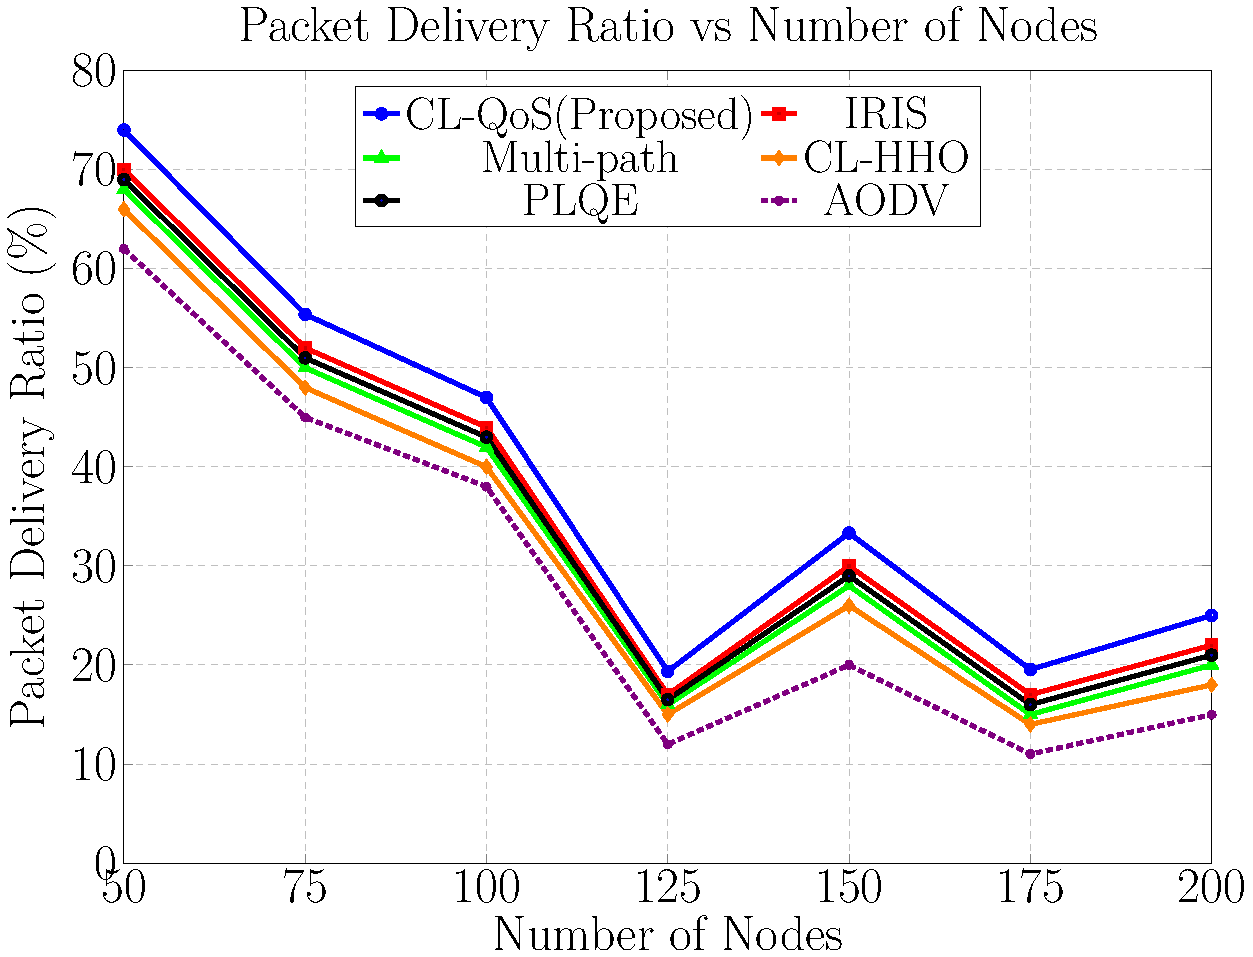
\includegraphics[width=0.48\textwidth]{figures/res1.pdf}
\captionof{figure}{Packet Delivery Ratio versus Number of Nodes}
\label{fig:pdr_nodes}
\end{center}
Figure~\ref{fig:pdr_nodes} shows that the packet delivery ratio decreases from approximately 74\% at 50 nodes to around 25\% at 200 nodes for the proposed CL-QoS model. In comparison, AODV drops below 20\% at higher node density. The proposed model consistently maintains higher delivery ratio than IRIS, Multi-path, CL-HHO, and PLQE. The performance gap increases at higher node counts, indicating better congestion handling and reliability of the proposed approach.

\vspace{0.3cm}

\begin{center}
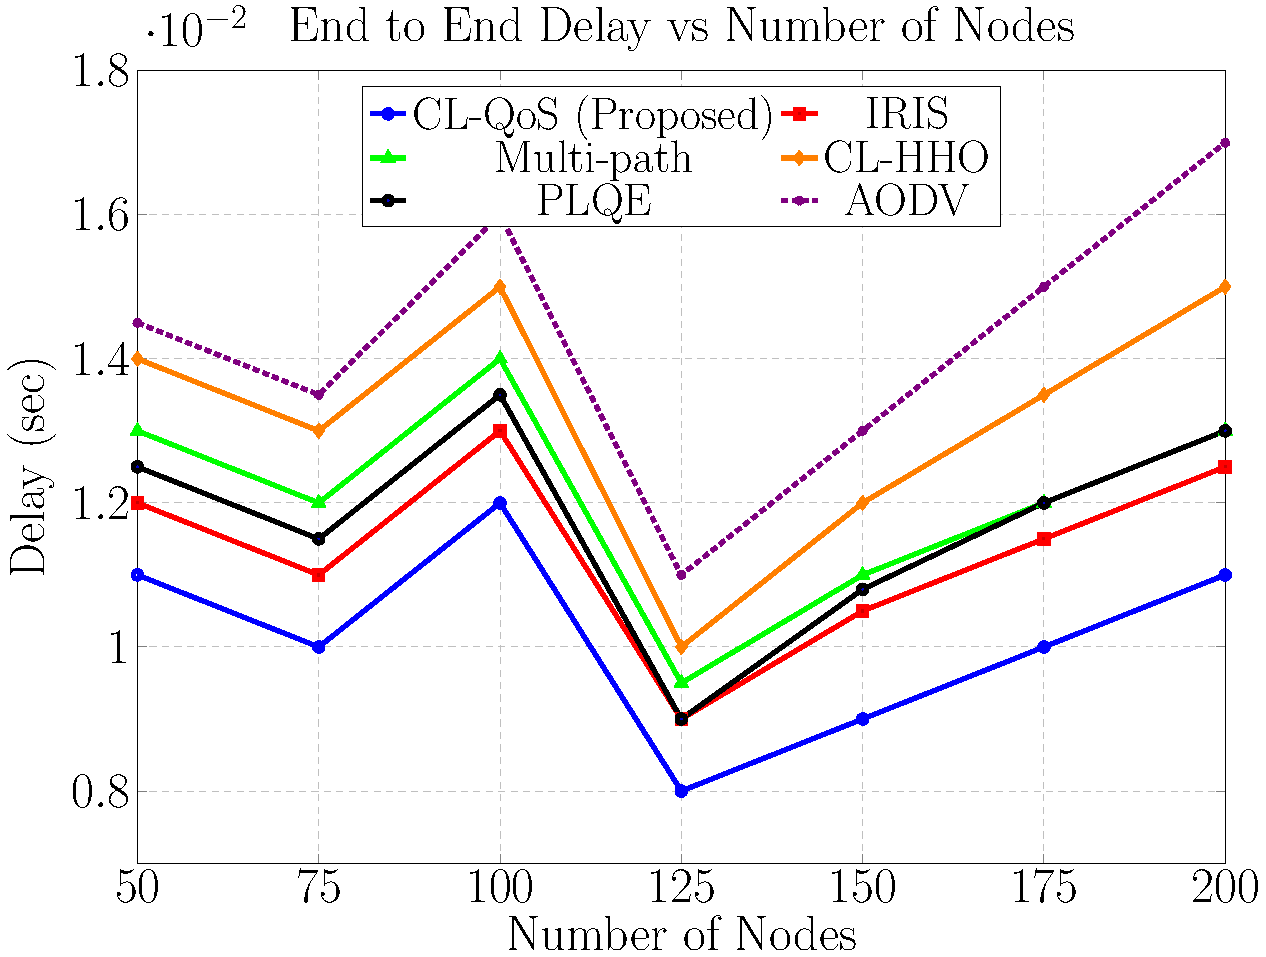
\includegraphics[width=0.48\textwidth]{figures/res2.pdf}
\captionof{figure}{End to End Delay versus Number of Nodes}
\label{fig:delay_nodes}
\end{center}
Figure~\ref{fig:delay_nodes} shows that the delay of the proposed model varies between 0.006 s and 0.013 s as node count increases from 50 to 200. In contrast, AODV exhibits higher delay reaching approximately 0.017 s. The proposed CL-QoS model consistently maintains lower delay compared to other methods, demonstrating efficient routing and reduced congestion effects at higher node densities.

\vspace{0.3cm}

\begin{center}
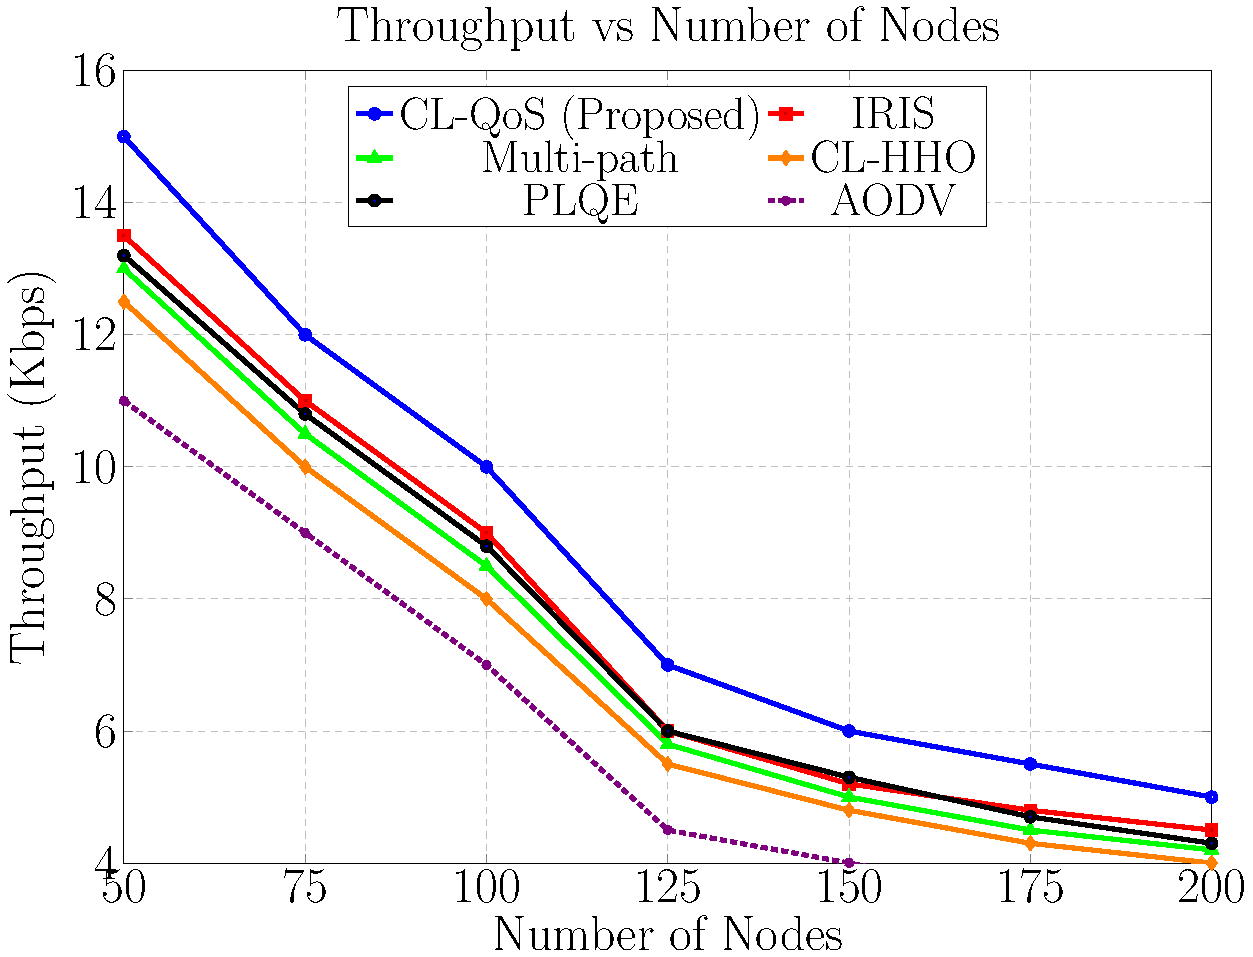
\includegraphics[width=0.48\textwidth]{figures/res3.pdf}
\captionof{figure}{Throughput versus Number of Nodes}
\label{fig:throughput_nodes}
\end{center}
Figure~\ref{fig:throughput_nodes} shows that throughput decreases from approximately 15 Kbps at 50 nodes to around 5 Kbps at 200 nodes for the proposed model. AODV shows lower throughput values, dropping below 4 Kbps at higher node counts. The proposed CL-QoS model maintains higher throughput across all node densities, indicating better packet delivery efficiency.

\vspace{0.3cm}

\begin{center}
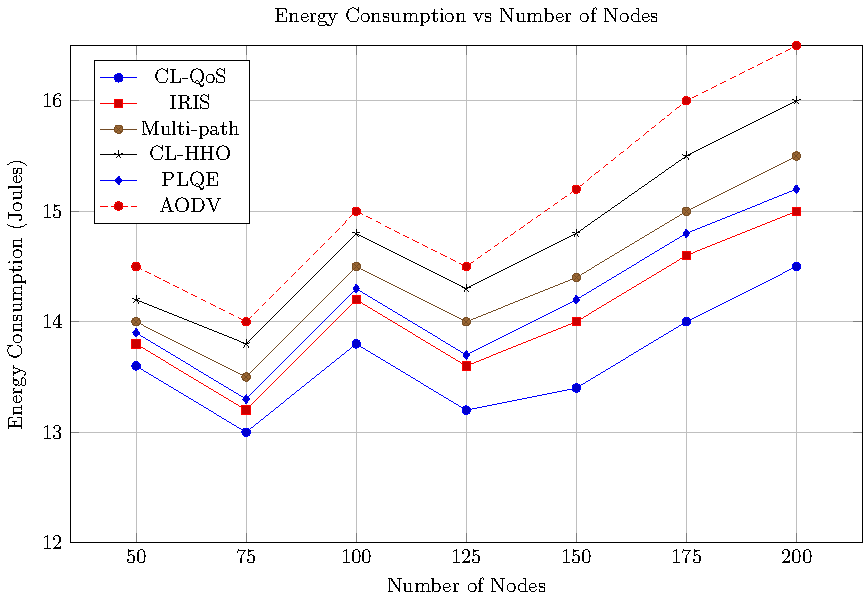
\includegraphics[width=0.48\textwidth]{figures/res4.pdf}
\captionof{figure}{Energy Consumption versus Number of Nodes}
\label{fig:energy_nodes}
\end{center}
Figure~\ref{fig:energy_nodes} shows that energy consumption increases from approximately 13.6 J at 50 nodes to around 14.5 J at 200 nodes for the proposed model. In comparison, AODV reaches above 16 J at higher node density. The proposed CL-QoS model consistently consumes less energy than other protocols, demonstrating improved energy efficiency.

\vspace{0.3cm}

\begin{center}
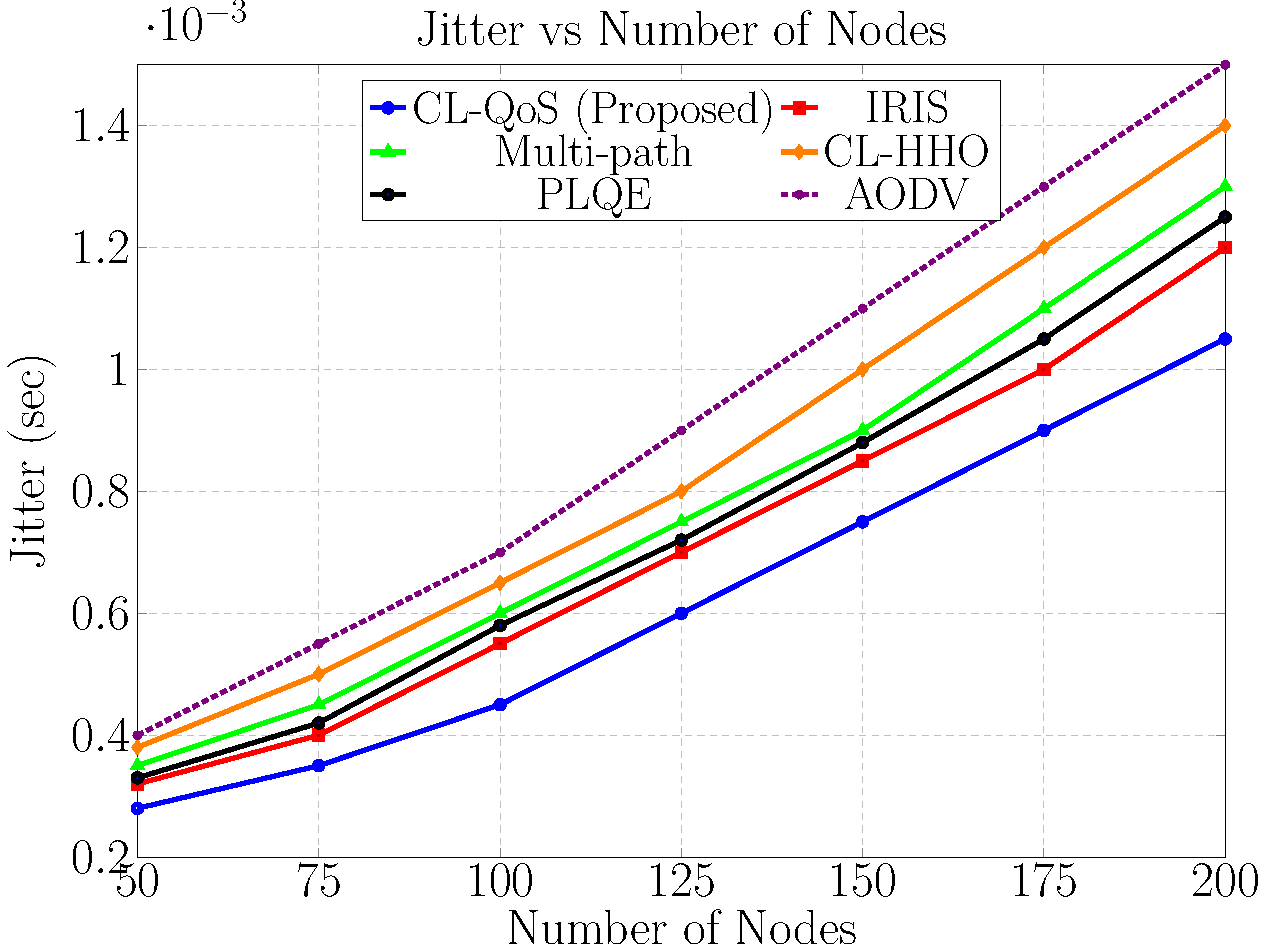
\includegraphics[width=0.48\textwidth]{figures/res5.pdf}
\captionof{figure}{Jitter versus Number of Nodes}
\label{fig:jitter_nodes}
\end{center}

Figure~\ref{fig:jitter_nodes} illustrates the variation of jitter with respect to the number of nodes. It is observed that jitter fluctuates due to dynamic network conditions such as congestion and retransmissions. The proposed CL-QoS model maintains relatively lower jitter compared to other methods, ensuring more stable packet delivery and improved communication quality.

\vspace{0.3cm}

\begin{center}
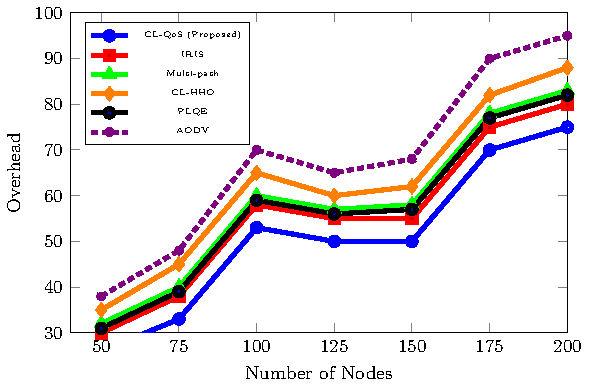
\includegraphics[width=0.48\textwidth]{figures/res6.pdf}
\captionof{figure}{Communication Overhead versus Number of Nodes}
\label{fig:overhead_nodes}
\end{center}
Figure~\ref{fig:overhead_nodes} shows that communication overhead increases from 26 units at 50 nodes to 75 units at 200 nodes for the proposed model. In contrast, AODV reaches approximately 95 units. The proposed CL-QoS model maintains lower overhead compared to other protocols, indicating efficient routing control.


\subsection{Performance Analysis}

\begin{center}
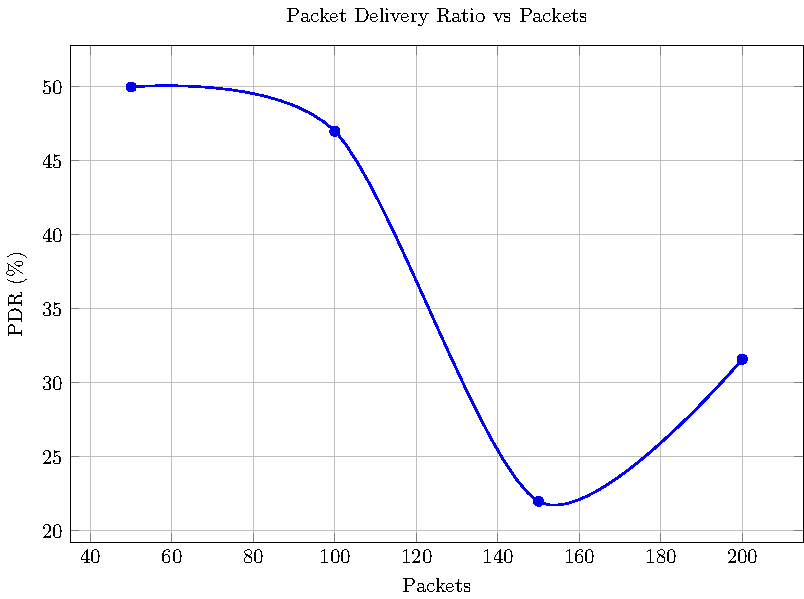
\includegraphics[width=0.48\textwidth]{figures/res7.pdf}
\captionof{figure}{Packet Delivery Ratio versus Packets Sent}
\label{fig:pdr_packets}
\end{center}
Figure~\ref{fig:pdr_packets} shows that the packet delivery ratio decreases from approximately 50\% at 50 packets to about 31.6\% at 200 packets. A sharp drop is observed between 100 and 150 packets where the value reduces from around 47\% to nearly 22\%, indicating severe congestion and packet loss. Beyond this point, a slight recovery is seen due to adaptive routing behavior. Overall, the trend confirms that increased traffic load negatively impacts delivery performance, but the proposed CL-QoS model maintains reasonable stability under high traffic conditions.

\vspace{0.3cm}

\begin{center}
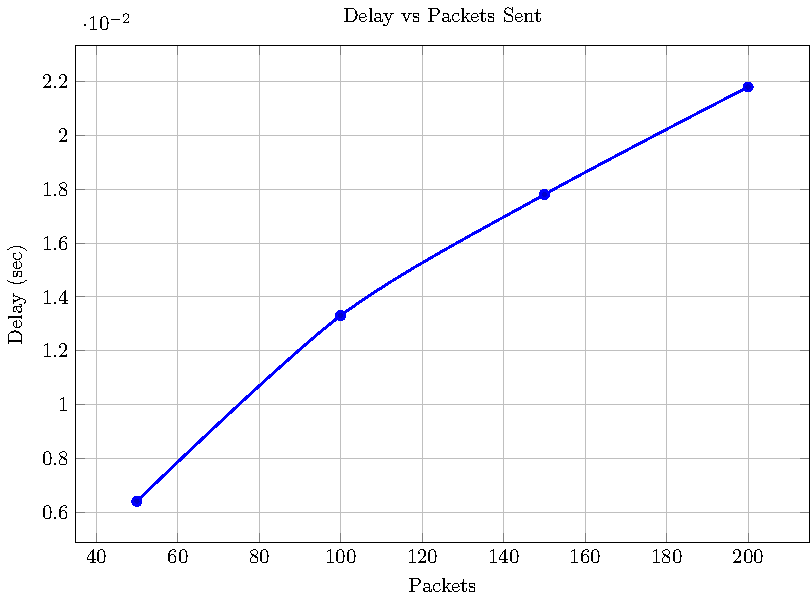
\includegraphics[width=0.48\textwidth]{figures/res8.pdf}
\captionof{figure}{Delay versus Packets Sent}
\label{fig:delay_packets}
\end{center}
Figure~\ref{fig:delay_packets} shows that delay increases steadily from approximately 0.006 s at 50 packets to about 0.022 s at 200 packets. The growth is gradual up to 100 packets and becomes more significant beyond that point due to increased queueing delay and network contention. The near-linear increase indicates that delay is directly influenced by traffic load. This behavior reflects typical network conditions where higher packet rates result in increased transmission latency and processing overhead.

\vspace{0.3cm}

\begin{center}
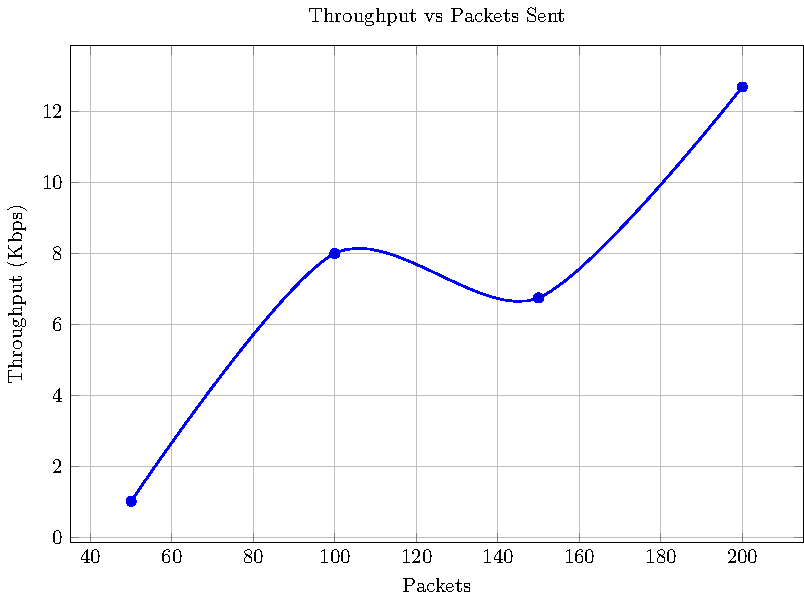
\includegraphics[width=0.48\textwidth]{figures/res9.pdf}
\captionof{figure}{Throughput versus Packets Sent}
\label{fig:throughput_packets}
\end{center}

Figure~\ref{fig:throughput_packets} illustrates that throughput increases from approximately 1 Kbps at 50 packets to nearly 12.7 Kbps at 200 packets. A significant rise is observed between 50 and 100 packets, after which throughput fluctuates slightly before reaching peak values. The variation around 150 packets indicates temporary congestion effects. Overall, the trend shows improved channel utilization with increasing packet transmission, demonstrating that the network effectively handles higher traffic up to a certain limit.

\vspace{0.3cm}

\begin{center}
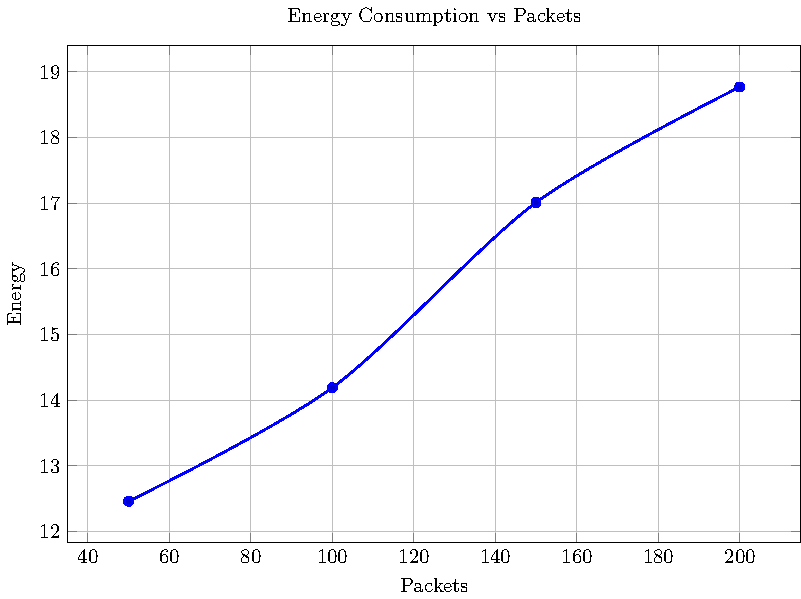
\includegraphics[width=0.48\textwidth]{figures/res10.pdf}
\captionof{figure}{Energy Consumption versus Packets}
\label{fig:energy_packets}
\end{center}

Figure~\ref{fig:energy_packets} shows that energy consumption increases from approximately 12.4 J at 50 packets to about 18.7 J at 200 packets. The increase is gradual initially and becomes more pronounced beyond 100 packets due to higher transmission and reception activities. The nearly linear growth indicates consistent energy usage with increasing traffic. This behavior confirms that energy consumption is directly proportional to packet load in the network.

\vspace{0.3cm}

\begin{center}
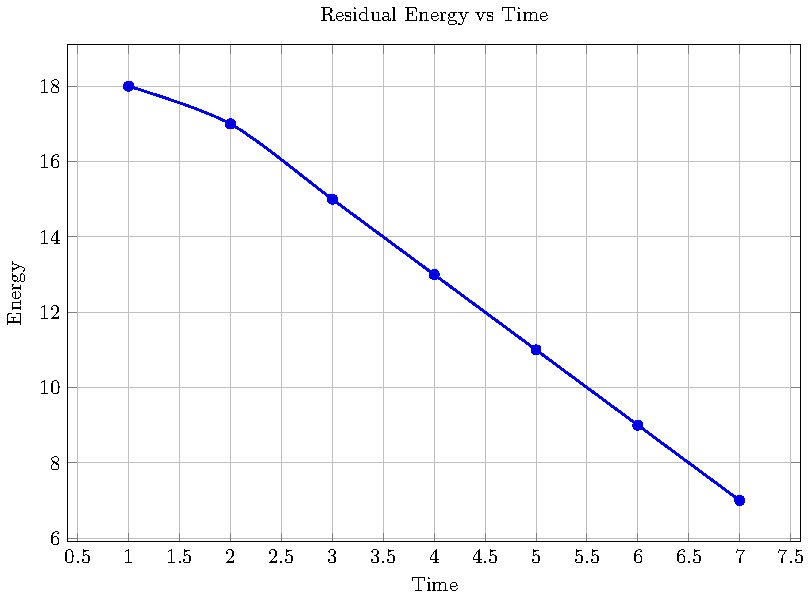
\includegraphics[width=0.48\textwidth]{figures/res11.pdf}
\captionof{figure}{Residual Energy versus Time}
\label{fig:energy_time}
\end{center}
Figure~\ref{fig:energy_time} shows that residual energy decreases steadily from approximately 18 J at the beginning to nearly 6 J at later time intervals. The reduction is gradual in the initial phase and becomes steeper as time progresses due to continuous data transmission and processing. The consistent downward trend indicates stable energy consumption over time without abrupt depletion. This reflects efficient energy utilization in the network.

\vspace{0.3cm}

\begin{center}
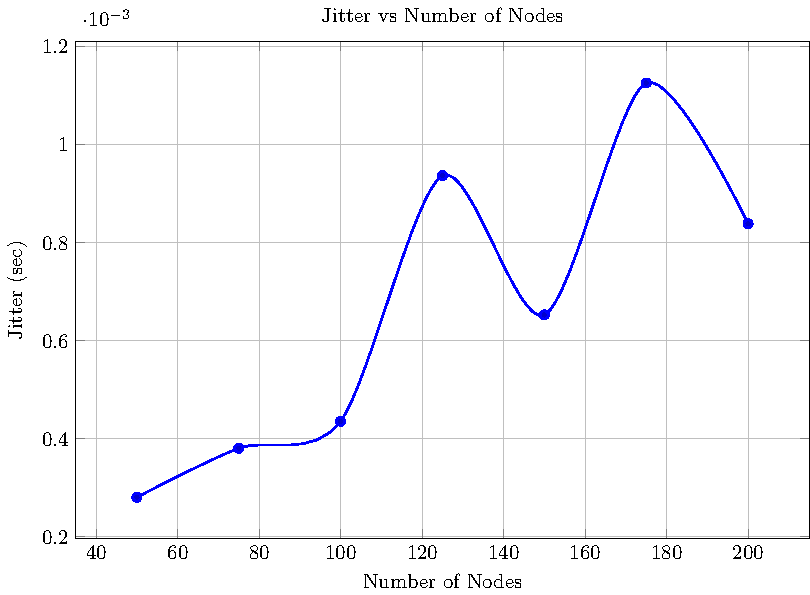
\includegraphics[width=0.48\textwidth]{figures/res12.pdf}
\captionof{figure}{Jitter versus Number of Nodes}
\label{fig:jitter_nodes_internal}
\end{center}

Figure~\ref{fig:jitter_nodes_internal} illustrates the variation of jitter with respect to the number of nodes. As node density increases, jitter generally rises and exhibits noticeable fluctuations due to dynamic congestion, variable queuing delays, and packet retransmissions. The jitter ranges approximately from 0.0002 s to 0.0012 s, with prominent spikes observed around 125 and 175 nodes, indicating periods of higher network congestion. Following these peaks, a slight reduction suggests temporary stabilization in delay variation. Overall, the results highlight the sensitivity of jitter to changing traffic conditions, while the proposed CL-QoS model effectively maintains controlled jitter levels within acceptable limits, ensuring stable communication performance and improved quality of service.

\section{Conclusion and Future Work}
The proposed Cross Layer QoS Adaptive Decision Support System provides an effective approach for improving reliability and performance in wireless sensor network based Internet of Things environments. By integrating cross layer parameters such as residual energy, link quality, delay, and traffic load, the system enables intelligent and adaptive routing decisions under dynamic network conditions. The multi metric cost function supports optimal path selection by balancing energy efficiency, communication reliability, and overall network performance. Simulation results demonstrate improvements in packet delivery ratio, delay, and throughput while maintaining controlled energy consumption and communication overhead. The adaptive routing mechanism effectively responds to congestion, link degradation, and varying traffic conditions.Overall, the proposed framework achieves improved Quality of Service and extends network lifetime compared to conventional approaches, making it suitable for large scale IoT applications.

Future work can focus on extending the proposed model to support node mobility and dynamic network conditions. The integration of intelligent techniques such as machine learning can further enhance routing decisions through predictive analysis. Additionally, the framework can be evaluated in large scale real time deployment scenarios and integrated with advanced IoT architectures to improve scalability, robustness, and adaptability.



\section*{Declarations}
\subsection*{Ethical Approval}
This manuscript reports studies that do not involve human participants, human data, human tissue, or animals.

\subsection*{Conflict of Interest}
The authors have no conflict of interest to declare that are relevant to the content of this article.

\subsection*{Authors' Contributions}
S. Gopikrishnan contributed to the conceptualization, Formal analysis, drafting the original manuscript, and designing the experimental protocols. Author-2 was responsible for Conceptualization, methodology, software implementation, and dataset curation. Author3 contributed to conceptualization, supervision, and in-depth analysis of the experimental results. Author-3 handled the review and editing of the final draft, as well as the overall validation of the study results.


\subsection*{Funding}
The authors did not receive financial support from any organization for the submitted work.

\subsection*{Availability of data and materials}
Data sharing is not applicable to this article, as no new data were created or analyzed in this study.

\subsection*{Acknowledgment}
We acknowledge that the hardware utilized in this research for evaluation is a part of the Intel IoT Center for Excellence, VIT-AP University. 

\bibliographystyle{cas-model2-names}
\bibliography{references}


\end{document}

